\documentclass{article}

\renewcommand{\familydefault}{\sfdefault}  %serifenlose Schrift
\usepackage{helvet} % Schrift: Helvetica


\usepackage{graphicx,graphics,tikz}
\usepackage{amsmath}
\usepackage{amsthm}
\usepackage{amsfonts}
\usepackage{amssymb}
\usepackage{marvosym} % to be able to show male and female symbols with: \Female and \Male
\usepackage{gensymb}
\usepackage[graphics,tightpage,active]{preview}
\definecolor{spain}{rgb}{0.2,0.87,0.93}
\definecolor{france}{rgb}{0.4,0.2,0.6}
\definecolor{denmark}{rgb}{1,0.87,0.07}
\definecolor{norway}{rgb}{0.2,0.4,0}

\PreviewEnvironment{tikzpicture}
\newlength\imagewidth
\newlength\imagescale

\begin{document}

%\pgfmathsetlength{\imagewidth}{10cm} % desired displayed width of image
%\pgfmathsetlength{\imagescale}{\imagewidth/2000} % pixel width of image
% adjust scale of tikzpicture (and direction of y) such that pixel
% coordinates can be used for drawing overlays:
\usetikzlibrary{backgrounds}

\begin{tikzpicture}
  \scalebox{0.9}{
\begin{scope}
\node [inner sep=0pt,outer sep=0pt] at (0cm,0cm) {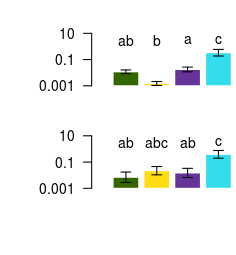
\includegraphics[width=4cm]{Controls_Comparisons.png}};
\draw[color=red,line width=0.03cm] (1.75cm,0.2cm) ellipse (0.5cm and 1.6cm);
\begin{scope}[xshift=1cm,yshift=1.7cm]
\draw [color=black,text centered,text width=10cm,anchor=west] (-2cm,0.8cm) node {\small{Constitutive \textit{shsp} gene expression before heat shock}};
\draw [color=black,text centered,text width=3cm,anchor=west] (-1.5cm,0.1cm) node {\scriptsize{23 weeks acclimation}};
\draw [color=black,text centered,text width=3cm,anchor=west] (-1.5cm,-1.5cm) node {\scriptsize{7 weeks acclimation}};
\draw [color=black,text centered,text width=3cm,anchor=west] (-2.8cm,-3cm) node [rotate=90] {\scriptsize{Normalized expression}};
\draw [color=red!90!black,text centered,text width=4cm,anchor=west] (6cm,-2.5cm) node {\small{High constitutive\\ stress}};
\node[anchor=north west,inner sep=0pt,outer sep=0pt,scale=1] at (3.5,0) {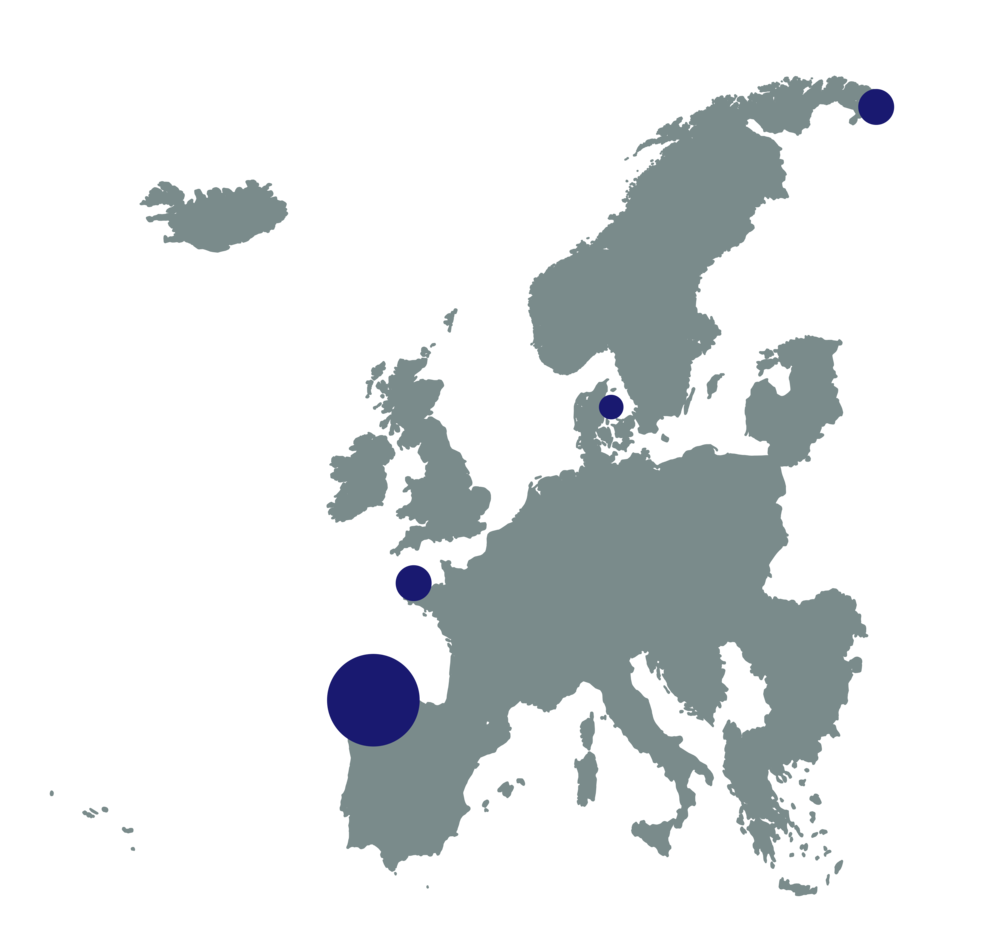
\includegraphics[width=3.5cm]{ConstitutiveHSP_r.png}};
\begin{scope}[xshift=1.5cm, yshift=0.5cm]
\draw [color=norway,fill=norway] (5.07,-0.87cm) circle (0.07cm);
\draw [color=denmark,fill=denmark] (4.15,-1.9cm) circle (0.06cm);
\draw [color=france,fill=france] (3.44,-2.56cm) circle (0.07cm);
\draw [color=spain,fill=spain] (3.3,-2.95cm) circle (0.18cm);
\end{scope}
\begin{scope}[xshift=1.3cm,yshift=0.4cm]
\draw [color=black](5,-1.25+0.8) node {\small{Norway}};
\draw [color=black](3.7-1,-1.85) node {\small{Denmark}};
\draw [color=black](3.58-0.7,-2.43) node {\small{Brittany}};
\draw [color=black](3.4-0.7,-2.82) node  {\small{Spain}};
\end{scope}
\end{scope}
\end{scope}
}

\scalebox{0.9}{
\begin{scope}[yshift=-4.5cm]
\node [inner sep=0pt,outer sep=0pt] at (0cm,0cm) {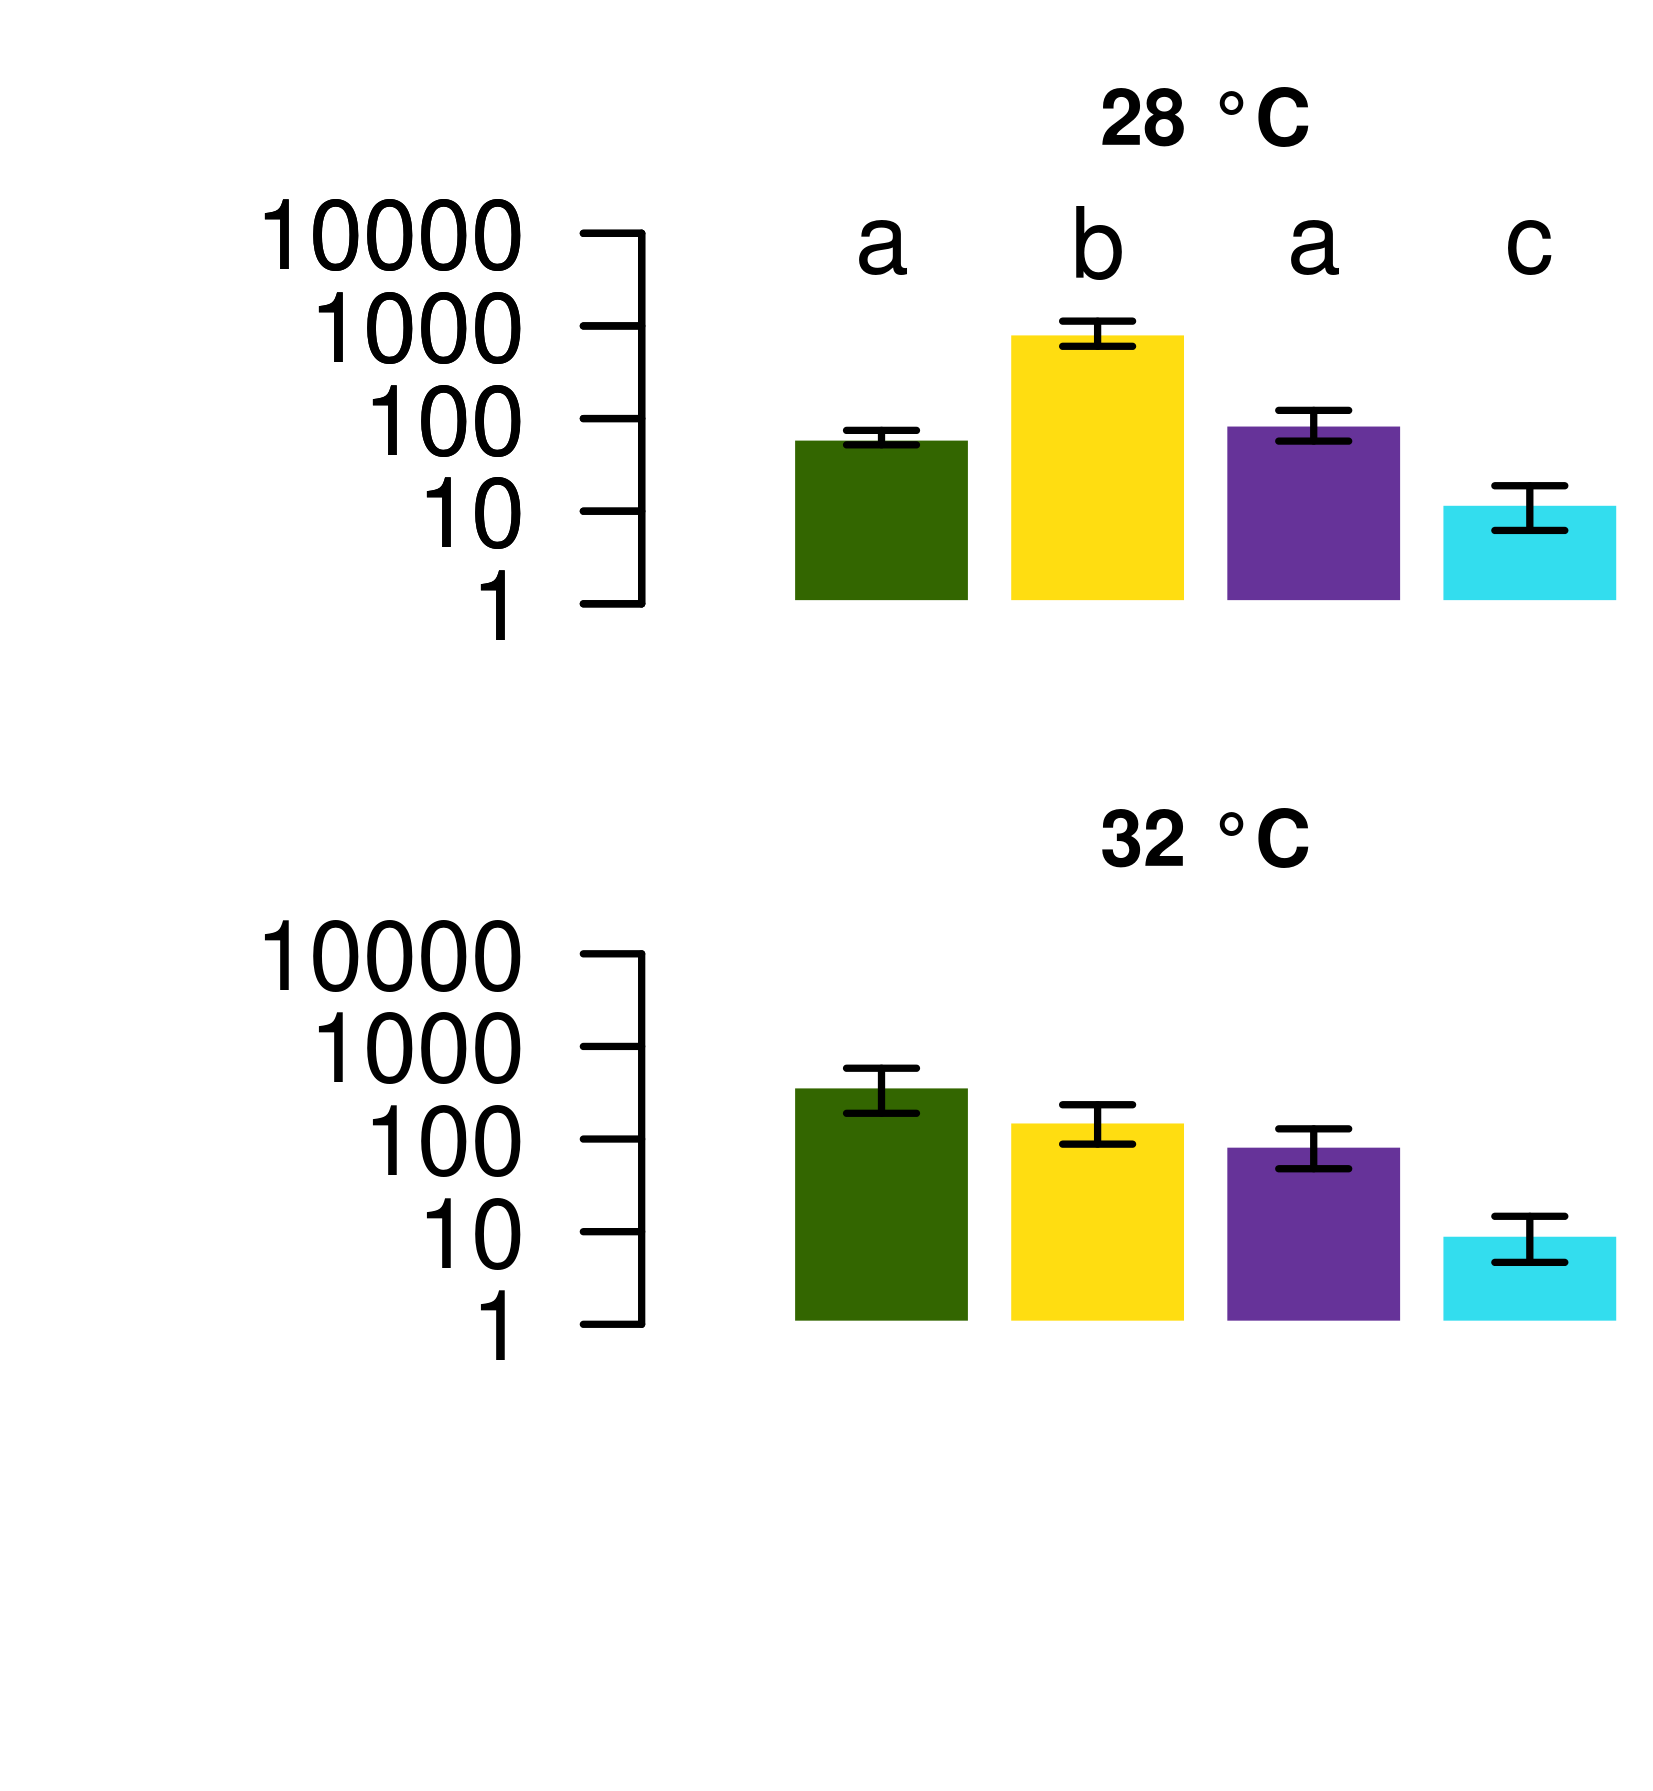
\includegraphics[width=4cm]{TreatmentComparisonsSHSP.png}};
\draw[color=red,line width=0.03cm] (1.75cm,0.2cm) ellipse (0.5cm and 1.6cm);
\begin{scope}[xshift=1cm,yshift=1.7cm]
\draw [color=black,text centered,text width=10cm,anchor=west] (-2cm,0.8cm) node {\small{Heat shock response of \textit{shsp} gene expression after 24h recovery}};
\draw [color=black,text centered,text width=3cm,anchor=west] (-2.8cm,-3cm) node [rotate=90] {\scriptsize{Fold change}};
\draw [color=red!90!black,text centered,text width=4cm,anchor=west] (6cm,-2.5cm) node {\small{Reduced\\ responsiveness}};
\node[anchor=north west,inner sep=0pt,outer sep=0pt,scale=1] at (3.5,0) {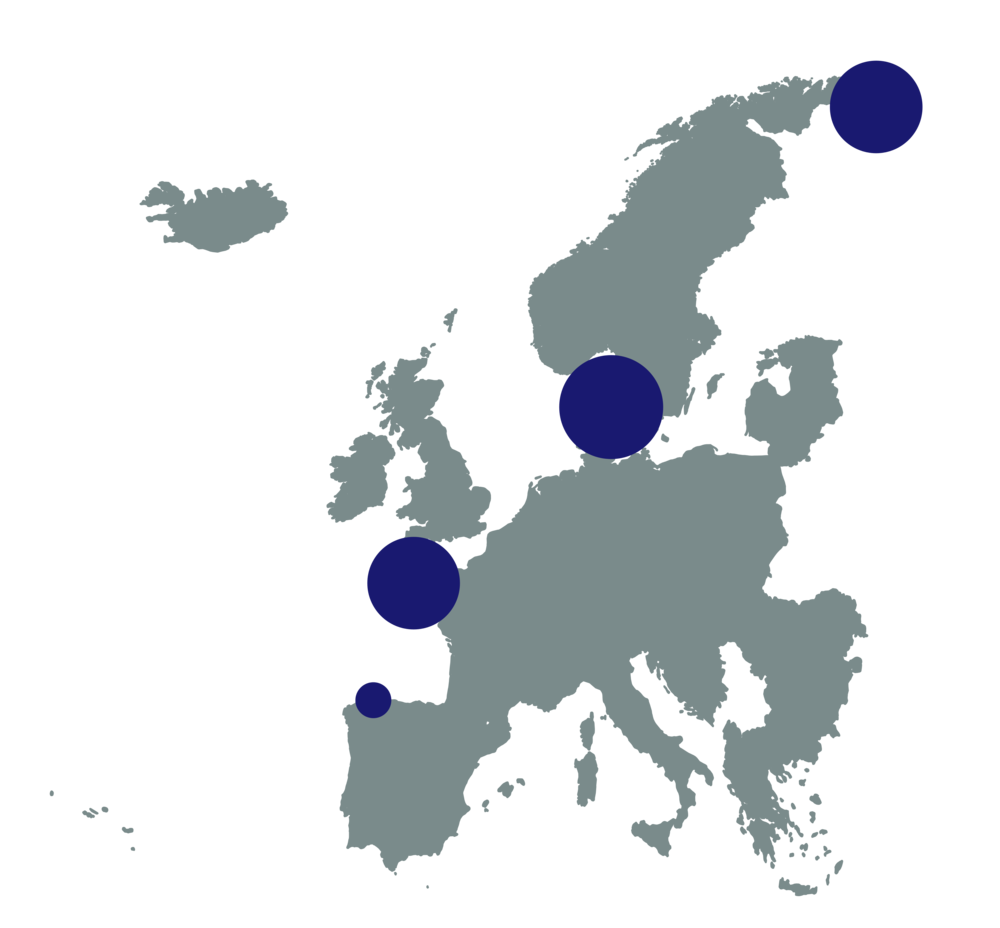
\includegraphics[width=3.5cm]{InducibleHSP_r.png}};
\begin{scope}[xshift=1.5cm, yshift=0.5cm]
\draw [color=norway,fill=norway] (5.07,-0.87cm) circle (0.18cm);
\draw [color=denmark,fill=denmark] (4.14,-1.92cm) circle (0.18cm);
\draw [color=france,fill=france] (3.44,-2.56cm) circle (0.18cm);
\draw [color=spain,fill=spain] (3.3,-2.95cm) circle (0.06cm);
\end{scope}
\begin{scope}[xshift=1.3cm,yshift=0.4cm]
\draw [color=black](5,-1.25+0.8) node {\small{Norway}};
\draw [color=black](3.7-1,-1.85) node {\small{Denmark}};
\draw [color=black](3.58-0.7,-2.43) node {\small{Brittany}};
\draw [color=black](3.4-0.7,-2.82) node  {\small{Spain}};
\end{scope}
\end{scope}
\end{scope}
}



\end{tikzpicture}

\end{document}